\documentclass{beamer}

\usepackage[utf8]{inputenc}
\usepackage{default}
\usepackage{graphicx}
\usepackage{tikz}
\usetikzlibrary{shapes,arrows}

\usetheme{Warsaw}
\title{Financial privacy implications of cryptocurrencies}
\author{Alice Townes, Richard Downe}

\begin{document}

% Define block styles
\tikzstyle{decision} = [diamond, draw, fill=blue!20, 
    text width=4.5em, text badly centered, node distance=3cm, inner sep=0pt]
\tikzstyle{block} = [rectangle, draw, fill=blue!20, 
    text width=5em, text centered, rounded corners, minimum height=4em]
\tikzstyle{line} = [draw, -latex']
\tikzstyle{cloud} = [draw, ellipse,fill=red!20, node distance=3cm,
    minimum height=2em]
    
\begin{frame}
 \titlepage
\end{frame}

\begin{frame}
 Bitcoin overview
 \begin{itemize}
  \item Entire supply is encoded in a lengthy cryptographic hash.
  \item Money changes hands when the owner of a quantity reassigns it by appending the register and cryptographically ``signing'' it.
  \item Ownership defined in terms of ``address'', a hash computed from a user's public key.
  \item Loss of the key used for signing constitutes a permanent loss of value from the supply.
  \item All transactions are visible to the public.
  \item Identities of users cannot directly be inferred from blockchain, without associating external data.
 \end{itemize}
\end{frame}
 
\begin{frame}
  View of the blockchain\\
  \vspace{1em}
  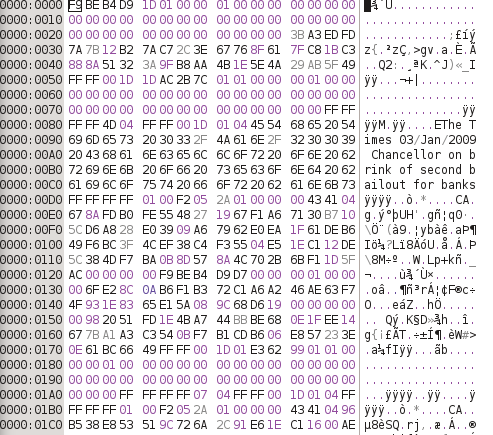
\includegraphics[height=0.7\textheight]{blockchain}
\end{frame}

\begin{frame}
 Anatomy of a bitcoin transaction\\
 \vspace{1em}
 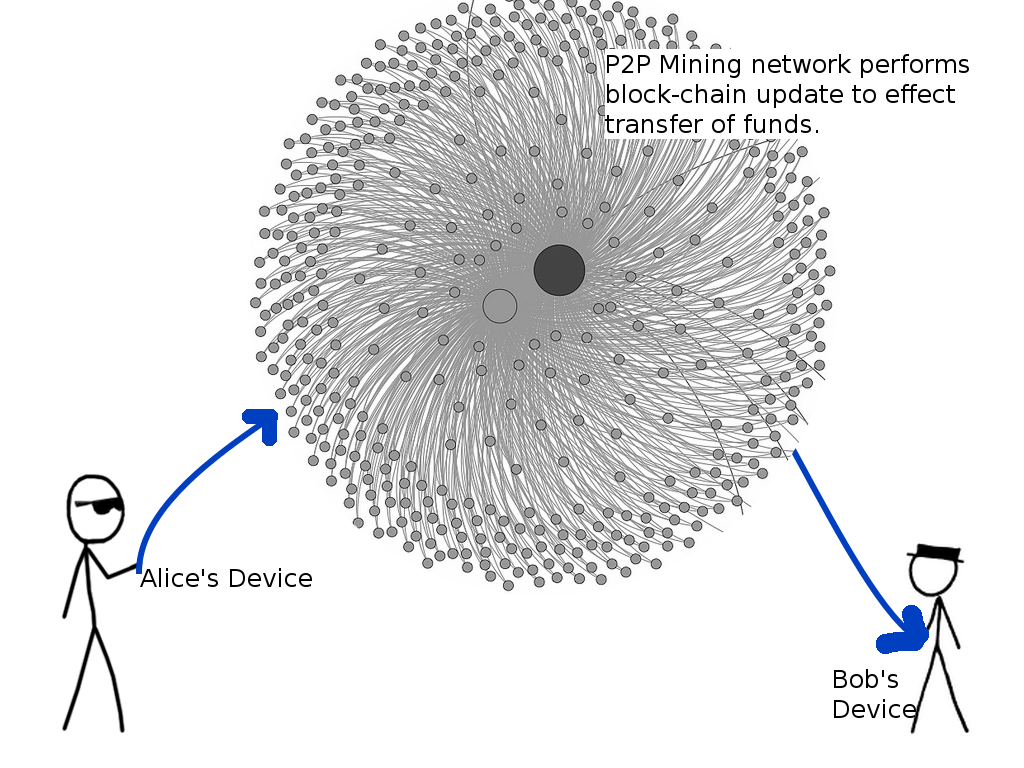
\includegraphics[width=0.8\textwidth]{AnatomyOfBitcoin}
\end{frame}

\begin{frame}
 Limitations of cryptography\\
 \vspace{1em}
 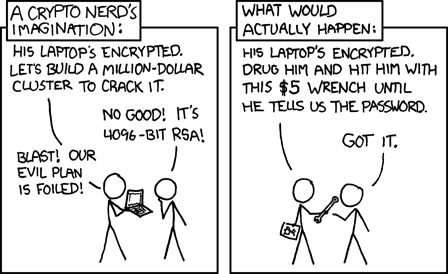
\includegraphics[width=0.8\textwidth]{security}
\end{frame}


\end{document}
